\documentclass[12 pt]{extarticle}

	\usepackage[frenchb]{babel}
	\usepackage[utf8]{inputenc}  
	\usepackage[T1]{fontenc}
	\usepackage{amssymb}
	\usepackage[mathscr]{euscript}
	\usepackage{stmaryrd}
	\usepackage{amsmath}
	\usepackage{tikz}
	\usepackage[all,cmtip]{xy}
	\usepackage{amsthm}
	\usepackage{varioref}
	\usepackage{geometry}
	\geometry{a4paper}
	\usepackage{lmodern}
	\usepackage{hyperref}
	\usepackage{array}
	 \usepackage{fancyhdr}
\renewcommand{\theenumi}{\alph{enumi})}
	\pagestyle{fancy}
	\theoremstyle{plain}
	\fancyfoot[C]{} 
	\fancyhead[L]{Contrôle}
	\fancyhead[R]{11 décembre 2023}\geometry{
 a4paper,
 total={170mm,257mm},
 left=20mm,
 top=20mm,
 }
	
	
	\title{Contrôle Chapitre 3}
	\date{}
	\begin{document}

\begin{center}{\Large Contrôle}\\ 
 \end{center}
 
 \subsection*{Exercice 1 - 3 points} 
 
 Recopier et compléter avec les symboles $<$, $>$, et $=$. 
 
 \[ 2,3 \ldots 2, 23 \hspace{2 cm}; \hspace{2 cm}
 3, 9740 \ldots 3, 974 \hspace{2 cm}; \hspace{2 cm}
 4,122 \ldots 4, 1221\]
 
 \subsection*{Exercice 2 - 4 points}
 
 Ranger dans l'ordre croissant les nombres suivants : 
 
 \[ 
 9 + \frac{2}{100} + \frac{1}{1000}; \hspace{2 cm}
 \frac{913}{100}; \hspace{2 cm}
 9,12    ; \hspace{2 cm}
 \frac{9112}{100} ; \hspace{2 cm}
 9 + \frac1{10} + \frac2{100} + \frac4{1000}
 \]
 
 \subsection*{Exercice 3 - 5 points}
 
 On considère le nombre $8 478, 936 78$. \begin{enumerate}
 \item Donner l'encadrement à l'unité. 
 \item Donner l'encadrement au centième. 
 \item Donner la valeur approchée au dixième par défaut. 
 \item Donner la valeur approchée au millième par excès. 
 \item Donner l'arrondi au dix-millième. 
 \end{enumerate}
 
 \subsection*{Exercice 4 - 4 points}
 
\begin{enumerate}

\item  Tracer un cercle de rayon $4$ cm et de centre $O$.
 \item Tracer une corde $[AB]$ de ce cercle. 
 \item Placer le point $C$ tel que $[AC]$ soit un diamètre du cercle.
 \item Quelle est la longueur $AC$ ? Justifier sans mesurer. 
\end{enumerate}
 \subsection*{Exercice 5 - 4 points}
 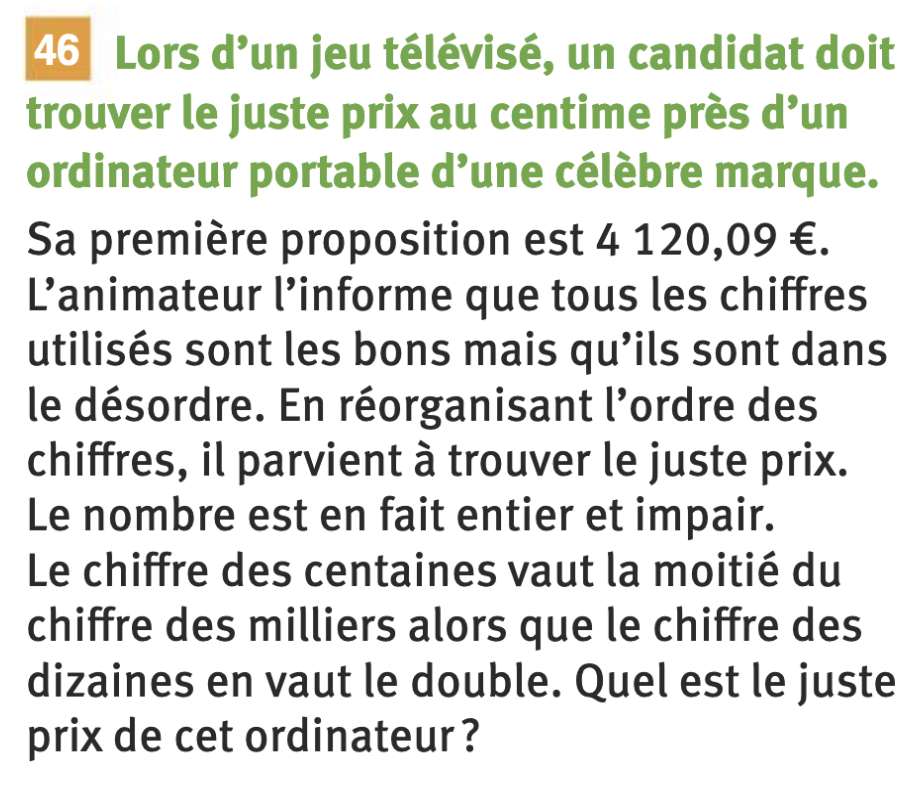
\includegraphics[scale=.6]{Exo5}
 
 \newpage
 

\begin{center}{\Large Contrôle}\\ 
 \end{center}
 
  \subsection*{Exercice 1 - 3 points} 
 
 Recopier et compléter avec les symboles $<$, $>$, et $=$. 
 
 \[ 5,309 \ldots 5, 3094 \hspace{2 cm}; \hspace{2 cm}
 65, 2330 \ldots 65, 233 \hspace{2 cm}; \hspace{2 cm}
 4,122 \ldots 4, 12\]
 
 \subsection*{Exercice 2 - 4 points}
 
 Ranger dans l'ordre croissant les nombres suivants : 
 
 \[ 
 6 + \frac{2}{100} + \frac{3}{1000}; \hspace{2 cm}
 \frac{633}{100}; \hspace{2 cm}
 6,32    ; \hspace{2 cm}
 \frac{6312}{100} ; \hspace{2 cm}
 6 + \frac3{10} + \frac2{100} + \frac4{1000}
 \]
 
 \subsection*{Exercice 3 - 5 points}
 
 On considère le nombre $5 623, 546 78$. \begin{enumerate}
 \item Donner l'encadrement à l'unité. 
 \item Donner l'encadrement au centième. 
 \item Donner la valeur approchée au dixième par défaut. 
 \item Donner la valeur approchée au millième par excès. 
 \item Donner l'arrondi au dix-millième. 
 \end{enumerate}
 
 \subsection*{Exercice 4 - 4 points}
 
\begin{enumerate}

\item  Tracer un cercle de rayon $3$ cm et de centre $O$.
 \item Tracer un diamètre $[AB]$ de ce cercle. 
 \item Placer un point $C$ tel que $[BC]$ soit un diamètre du cercle.
 \item Quelle est la longueur $OC$ ? Justifier sans mesurer. 
\end{enumerate}
 \subsection*{Exercice 5 - 4 points}
 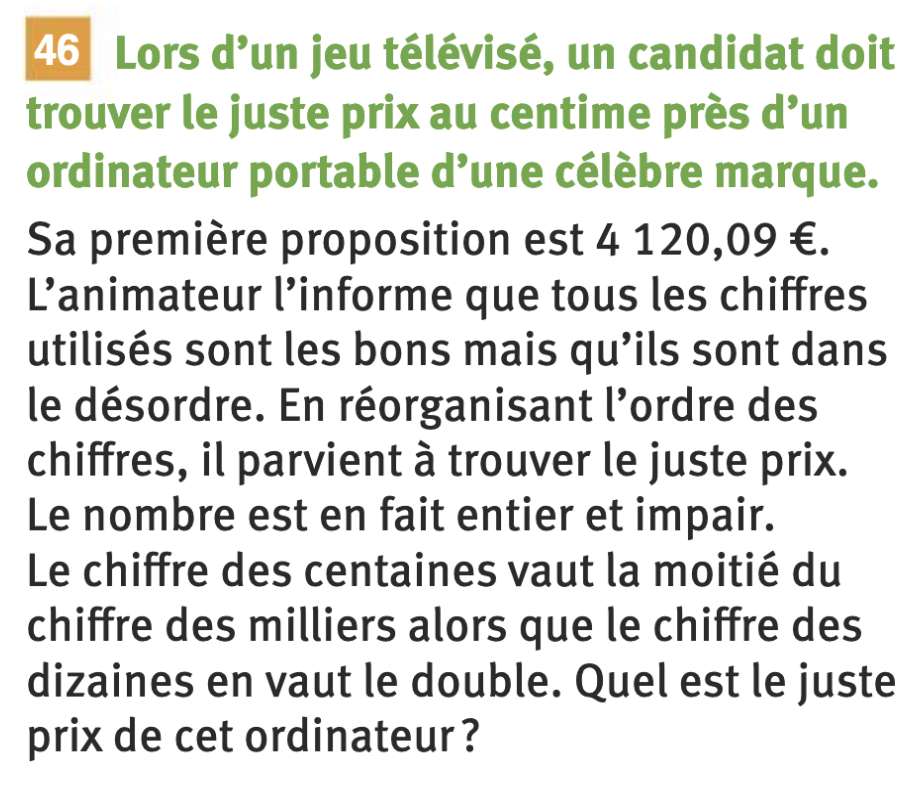
\includegraphics[scale=.6]{Exo5}
 	\end{document}
